% BU ASTRONOMY template for MS thesis and PhD dissertation.
%
%==========================================================================%
% MAIN PREAMBLE 
%==========================================================================%
%You may not have all of these packages installed.  If not, you may need to find them.  The files not included should be easily attainable through the usual latex channels.
\documentclass[12pt,letterpaper]{report}
\special{papersize=8.5in,11in}

%To skip a line between paragraphs
%\setlength{\parskip}{10pt plus 1pt minus 1pt}

\usepackage{epsfig, natbib}
\usepackage{stylefiles/aastex_hack}
\usepackage{fancyhdr,fancybox}
\usepackage{stylefiles/bu_astro_thesis}
%\usepackage{xspace}
\usepackage{indentfirst} %TO INDENT THE FIRST LINE OF A PARAGRAPH AT THE BEGINNING OF A NEW SECTION
%\usepackage{sidecap} %FOR CAPTIONS ON THE SIDE OF FIGURES
\usepackage{ulem} %FOR UNDERLINING AND SUCH
%\usepackage{url}
%\usepackage{wrapfig}
%\usepackage{amssymb}
\usepackage{longtable}
%\usepackage{multirow}

%%To get centered columns of a certain width
\usepackage{array}
\newcolumntype{x}[1]{%
>{\centering\hspace{0pt}}p{#1}}%

\bibliographystyle{stylefiles/agu08_bbl_link} %Also available is the 'apj' style (no titles)


%TO MAKE SURE MARGINS DON'T GET IGNORED
\widowpenalty=10000
\clubpenalty=10000
\setlength\parindent{2.2 em}
\raggedbottom
\tolerance=10000 %line break tolerances

% UNITS
\newcommand{\m}{$\,{\rm m}$}
\newcommand{\cm}{$\,{\rm cm}$}
\newcommand{\K}{\ensuremath{\,{\rm K}}}
\newcommand{\ks}{${\,{\rm km\, sec^{-1}}}$}
\newcommand{\msun}{$\,M_{S}$}
\newcommand{\rsun}{$\,R_{S}$}
\newcommand{\percc}{\ensuremath{\,{\rm cm^{-3}}}}
\newcommand{\hr}{$\,{\rm hr}$}
\newcommand{\kms}{\ensuremath{\,{\rm km\,s}^{-1}}}
\newcommand{\degper}{\ensuremath{\rlap.{^{\circ}}}}
\newcommand{\rearth}{R$_{E}$}
\newcommand{\degrees}{$^{\circ}$}

%%FOR SUB AND SUPERSCRIPTS IN TEXT
\newcommand{\superscript}[1]{\ensuremath{^{\textrm{#1}}}}
\newcommand{\subscript}[1]{\ensuremath{_{\textrm{#1}}}}

%%TO ALIGN TABLE ROWS THAT ARE UNDER A HORIZONTAL LINE
\newcommand{\topline}{\rule{0pt}{2.3ex}}
\newcommand{\bottomline}{\rule[-1.2ex]{0pt}{0pt}}


%#############################
%THIS ONE IS VERY USEFUL!!!!!
%#############################
\setkeys{Gin}{draft=False} %if True, all figures will print as just an empty box (useful when you don't want to wait for an entire dissertation with figures to compile)
%#############################
%#############################


\renewcommand{\topfraction}{0.75}	% max fraction of floats at top
\renewcommand{\bottomfraction}{0.1}	% max fraction of floats at bottom

%Parameters for TEXT pages (not float pages):
\setcounter{topnumber}{2}
\setcounter{bottomnumber}{2}
\setcounter{totalnumber}{4}     % 2 may work better
\renewcommand{\textfraction}{0.07}	% allow minimal text w. figs
%Parameters for FLOAT pages (not text pages):
\renewcommand{\floatpagefraction}{0.7}	% require fuller float pages
% N.B.: floatpagefraction MUST be less than topfraction !!
\renewcommand{\dblfloatpagefraction}{0.7}	% require fuller float pages

%DEFINE WHAT THE BULLETS LOOK LIKE
\renewcommand{\labelitemi}{\textbullet} %FIRST LEVEL BULLET
\renewcommand{\labelitemii}{$\circ$} %SECOND LEVEL BULLET

%SO WE CAN USE \href AND \url
\usepackage[implicit=True,breaklinks=False,linktocpage=True,pdfborder={0 0 1},pdfborderstyle={/S/U/W 1},linkbordercolor={0 0 1},citebordercolor={0 0 1},filebordercolor={0 0 1},menubordercolor={0 0 1},runbordercolor={0 0 1},urlbordercolor={0 0 1},dvips]{hyperref}

%SET MARGINS
\setlength{\topmargin}{0.0in}
\setlength{\headheight}{.12in}
\setlength{\headsep}{0.33in}
\setlength{\textheight}{8.48in}
\setlength{\textwidth}{5.96in}
\setlength{\oddsidemargin}{0.52in}
\setlength{\evensidemargin}{0.52in}
\setlength{\footskip}{0.30in}


%==========================================================================%
%==========================================================================%
% BEGIN
%==========================================================================%
\begin{document}

%####################################################
%Preliminary Stuff
%####################################################
\title{YOUR TITLE HERE IN ALL CAPS}
\author{FIRST M LAST} %YOUR NAME
\degree=2 %2 = Doctor of Philisophy dissertation.
\prevdegrees{M.A., Boston University, Boston, MA, YYYY \\ B.S., Your Undergrad University, City, ST, YYYY}
\department{Department of Astronomy}
\defenseyear{YYYY}
\degreeyear{YYYY}
\reader{First}{First M. Reader, PhD}{Professor of Astronomy\\University of First Reader}
\reader{Second}{Second M. Reader, PhD}{Professor of Astronomy\\University of Second Reader}
\reader{Third}{Third M. Reader, PhD}{Title of Third Reader\\University of Third Reader}
\majorprof{First M. Reader}{\mbox{Professor of Astronomy.}}
\buecethesistitleboxpage %USUALLY COMMENT THIS LINE OUT
\maketitle
\copyrightpage %USUALLY COMMENT BELOW OUT (INCLUSIVE OF THIS LINE)
\approvalpage
\newpage
\chapter*{Acknowledgments}
\input{extras/acknowledgements}
\begin{abstractpage}
\input{extras/abstract}
\end{abstractpage}  %USUALLY COMMENT ABOVE OUT (INCLUSIVE OF THIS LINE)
\tableofcontents
\newpage	
\listoftables
\newpage
\listoffigures
% List of Abbrevs is NOT optional (Martha Wellman likes all abbrevs listed)
\chapter*{List of Abbreviations}
\begin{center}
  \begin{longtable}{lll}
%    \hspace*{2em} & \hspace*{1in} & \hspace*{4.5in} \\
    TLA  & ~~~~~ & Three Letter Acronym \\
    OAH  & ~~~~~ & Other Acronyms Here \\
  \end{longtable}
\end{center}
\newpage
\endofprelim

%####################################################
%THE REAL CONTENT
%####################################################

%\setcounter{chapter}{2} %If I was printing off only chapter 3 (for example), then I would comment out the other chapter directly below here and use this line to make the chapter count correct

\chapter{Chapter title}
\label{sec:firstchap}
\thispagestyle{myheadings}

Example reference to Section \ref{sec:fakesection}.  Example reference to Figure \ref{fig:fakefigure}.  Example parenthetical citation: \citep[e.g][for example]{gosling_1993}.   Example textual citation to \citet[][]{gosling_1993}.  

Lorem ipsum dolor sit amet, consectetur adipiscing elit. Praesent nec velit magna. In vehicula accumsan blandit. Duis vestibulum eros et ante posuere et pharetra nibh dapibus. Pellentesque quis nibh vestibulum urna fermentum convallis. Duis ultricies felis eget orci sodales sed varius ante facilisis. Vivamus nec lorem nulla. Donec id quam id arcu fringilla euismod. Etiam ullamcorper posuere ipsum, vel egestas ipsum bibendum faucibus. Proin volutpat dolor vel nulla egestas in ultricies mi pellentesque. Vivamus ut nulla ligula.

Vestibulum sed ante leo, et malesuada massa. Aenean vulputate dictum auctor. Nunc dignissim nibh ut lorem placerat eu convallis magna fermentum. Nullam ut magna in libero pharetra semper. Phasellus et odio sit amet eros facilisis dignissim. Curabitur tempor aliquet purus, ac blandit sem viverra ac. Vivamus non leo augue, ac semper orci. Integer non felis et arcu commodo tristique. Donec est justo, vehicula in dapibus quis, molestie nec elit. Mauris non congue neque. Duis id justo id lorem porta lobortis. Proin dapibus commodo interdum. Sed tincidunt lobortis nisl eu mollis.

%#################################################################################################
%#################################################################################################
%Section
%#################################################################################################
%#################################################################################################

\section{Second Section}
\label{sec:fakesection}
Lorem ipsum dolor sit amet, consectetur adipiscing elit. Praesent nec velit magna. In vehicula accumsan blandit. Duis vestibulum eros et ante posuere et pharetra nibh dapibus. Pellentesque quis nibh vestibulum urna fermentum convallis. Duis ultricies felis eget orci sodales sed varius ante facilisis. Vivamus nec lorem nulla. Donec id quam id arcu fringilla euismod. Etiam ullamcorper posuere ipsum, vel egestas ipsum bibendum faucibus. Proin volutpat dolor vel nulla egestas in ultricies mi pellentesque. Vivamus ut nulla ligula.

%#################################################################################################
%#################################################################################################

\subsection{Subsection}
\label{sec:fakesubsec}

\subsubsection*{Subsubsection}
Lorem ipsum dolor sit amet, consectetur adipiscing elit. Praesent nec velit magna. In vehicula accumsan blandit. Duis vestibulum eros et ante posuere et pharetra nibh dapibus. Pellentesque quis nibh vestibulum urna fermentum convallis. Duis ultricies felis eget orci sodales sed varius ante facilisis. Vivamus nec lorem nulla. Donec id quam id arcu fringilla euismod. Etiam ullamcorper posuere ipsum, vel egestas ipsum bibendum faucibus. Proin volutpat dolor vel nulla egestas in ultricies mi pellentesque. Vivamus ut nulla ligula.

\begin{figure}[!hbtp]
\centering
\includegraphics[height=\linewidth, angle=0]{chapter1/figures/bunny.ps}
\caption[Caption for `list of figures' page here]{Caption to be shown under the figure here}
\label{fig:fakefigure}
\end{figure}

\begin{equation}
\label{eqn:fakeequation}
R_{L} = \frac{mv_{\perp}}{qB}
\end{equation}

{\noindent}Lorem ipsum dolor sit amet, consectetur adipiscing elit. Praesent nec velit magna. In vehicula accumsan blandit. Duis vestibulum eros et ante posuere et pharetra nibh dapibus. Pellentesque quis nibh vestibulum urna fermentum convallis. Duis ultricies felis eget orci sodales sed varius ante facilisis. Vivamus nec lorem nulla. Donec id quam id arcu fringilla euismod. Etiam ullamcorper posuere ipsum, vel egestas ipsum bibendum faucibus. Proin volutpat dolor vel nulla egestas in ultricies mi pellentesque. Vivamus ut nulla ligula.  

\begin{table}[!htp]
\begin{center}
\begin{tabular*}{.75\textwidth}{@{\extracolsep{\fill}} c  c  c  c}
    \hline
    \topline Energy & Velocity & $R_{L}$ (Earth Radii) & $R_{L}$ (AU)\tabularnewline
    \hline
    \topline 
	10 MeV & 0.14c & 14 & 0.0006\tabularnewline
	100 MeV & 0.43c & 46 & 0.0002\tabularnewline
	1 GeV & 0.87c & 176 & 0.007\tabularnewline
	100 GeV & 0.99c & 10400 & 0.4\tabularnewline
    \hline
\end{tabular*}
\caption[Caption for `List of Tables' here]{Caption to be shown under table here}
\label{tab:faketable}
\end{center}
\end{table}

\include{chapter2/chapter2}
\include{chapter3/chapter3}
\chapter{Chapter 4 Title}
\label{sec:chap4}
\thispagestyle{myheadings}

\section{This Section Title}
\label{sec:thissec}

Lorem ipsum dolor sit amet, consectetur adipiscing elit. Praesent nec velit magna. In vehicula accumsan blandit. Duis vestibulum eros et ante posuere et pharetra nibh dapibus. Pellentesque quis nibh vestibulum urna fermentum convallis. Duis ultricies felis eget orci sodales sed varius ante facilisis. Vivamus nec lorem nulla. Donec id quam id arcu fringilla euismod. Etiam ullamcorper posuere ipsum, vel egestas ipsum bibendum faucibus. Proin volutpat dolor vel nulla egestas in ultricies mi pellentesque. Vivamus ut nulla ligula. 

%%###############################################################################################

\subsection{Subsection}
\label{sec:subsec}

Lorem ipsum dolor sit amet, consectetur adipiscing elit. Praesent nec velit magna. In vehicula accumsan blandit. Duis vestibulum eros et ante posuere et pharetra nibh dapibus. Pellentesque quis nibh vestibulum urna fermentum convallis. Duis ultricies felis eget orci sodales sed varius ante facilisis. Vivamus nec lorem nulla. Donec id quam id arcu fringilla euismod. Etiam ullamcorper posuere ipsum, vel egestas ipsum bibendum faucibus. Proin volutpat dolor vel nulla egestas in ultricies mi pellentesque. Vivamus ut nulla ligula. 
\chapter{Chapter 5 Title}
\label{sec:chap5}
\thispagestyle{myheadings}

\section{This Section Title}
\label{sec:thissec}

Lorem ipsum dolor sit amet, consectetur adipiscing elit. Praesent nec velit magna. In vehicula accumsan blandit. Duis vestibulum eros et ante posuere et pharetra nibh dapibus. Pellentesque quis nibh vestibulum urna fermentum convallis. Duis ultricies felis eget orci sodales sed varius ante facilisis. Vivamus nec lorem nulla. Donec id quam id arcu fringilla euismod. Etiam ullamcorper posuere ipsum, vel egestas ipsum bibendum faucibus. Proin volutpat dolor vel nulla egestas in ultricies mi pellentesque. Vivamus ut nulla ligula. 



% List of Abbreviated Journal Names  (Martha Wellman likes all abbrevs listed)
% This was in the preliminary pages before. But it should be just before the references according to Martha Khan.

\chapter*{List of Journal Abbreviations}

%\thispagestyle{empty}
\thispagestyle{myheadings}
%\thispagestyle{plain}

\begin{center}
  \begin{longtable}{lll}
%    \hspace*{2em} & \hspace*{1in} & \hspace*{4.5in} \\
	Ann. Geophys. & ~~~~~ & Annales Geophysicae \\
	Appl. Opt. & ~~~~~ & Applied Optics \\
	Astron. Astrophys. & ~~~~~ & Astronomy and Astrophysics \\
    Astrophys. J. & ~~~~~ & Astrophysical Journal \\
    Astrophys. J. Lett.  & ~~~~~ & Astrophysical Journal Letters \\
    Geophys. Monogr. & ~~~~~ & Geophysical Monograph \\
    Geophys. Res. Lett. & ~~~~~ & Geophysical Research Letters \\
    J. Atmos. Solar Terr. Phys. & ~~~~~ & Journal of Atmospheric and \\
    ~ & ~ &Solar-Terrestrial Physics \\
    J. Geophys. Res. & ~~~~~ & Journal of Geophysical Research \\
    Mon. Not. R. Astron. Soc. & ~~~~~ & Monthly Notices of the Royal \\
    ~ & ~ & Astronomical Society \\
	Nucl. Instrum. Methods  & ~~~~~ & Nuclear Instruments and Methods \\
	Phys. Rev. & ~~~~~ & Physical Review \\
	Rev. Geophys. Space Phys. & ~~~~~ & Reviews of Geophysics and Space Physics \\
	Sol. Phys.  & ~~~~~ &  Solar Physics \\
	Space Sci. Rev. & ~~~~~ & Space Science Reviews \\
	Space Wea. J. & ~~~~~ & Space Weather Journal \\
  \end{longtable}
\end{center}


% -------------------------------------
% Bibliography
% -------------------------------------
\newpage
\singlespace
\bibliography{ExampleBibliography} %Path to your bibliography file.  Could be a path to anywhere on your machine

\newpage  
\chapter*{Curriculum Vitae} %The way Martha wanted it...CV looks like a chapter heading (though no number)
\addcontentsline{toc}{chapter}{Curriculum Vitae}
{\noindent}{\Large Your M. Name} \\ %and then your name a little smaller.
\newline
\thispagestyle{myheadings}

Insert your CV here (without your name at the top...that is taken care of in thesis.tex).  Martha wanted it so that the `Curriculum Vitae' showed up as a normal chapter heading, with your name smaller below that (again...see the thesis.tex file for that stuff)

\end{document}
